%%%%%%%%%%%%%%%%%%%%%%%%%%%%%%%%%%%%%%%%%
% Important note:
% Chapter heading images should have a 2:1 width:height ratio,
% e.g. 920px width and 460px height.
%
%%%%%%%%%%%%%%%%%%%%%%%%%%%%%%%%%%%%%%%%%


%----------------------------------------------------------------------------------------
%	PACKAGES AND OTHER DOCUMENT CONFIGURATIONS
%----------------------------------------------------------------------------------------

\documentclass[openany,11pt,fleqn]{book} % Default font size and left-justified equations

\usepackage[top=3cm,bottom=3cm,left=3.2cm,right=3.2cm,headsep=10pt,letterpaper]{geometry} % Page margins

\usepackage{xcolor} % Required for specifying colors by name
\definecolor{ocre}{RGB}{52,177,201} % Define the orange color used for highlighting throughout the book

% Font Settings
\usepackage{avant} % Use the Avantgarde font for headings
%\usepackage{times} % Use the Times font for headings
\usepackage{mathptmx} % Use the Adobe Times Roman as the default text font together with math symbols from the Sym­bol, Chancery and Com­puter Modern fonts
\usepackage{microtype} % Slightly tweak font spacing for aesthetics
\usepackage[utf8]{inputenc} % Required for including letters with accents
\usepackage[T1]{fontenc} % Use 8-bit encoding that has 256 glyphs
\usepackage{amsthm}

\usepackage{mathtools}

\usepackage{minted}

\usepackage{tikz}
\usepackage{pgfplots}
\usepgfplotslibrary{fillbetween}
\usepackage{multirow}
\usepackage{array}
\usetikzlibrary{arrows.meta, positioning, calc, trees, shapes, decorations, matrix, fit}

% Bibliography
\usepackage[style=alphabetic,sorting=nyt,sortcites=true,autopunct=true,babel=hyphen,hyperref=true,abbreviate=false,backref=true,backend=biber]{biblatex}
\addbibresource{bibliography.bib} % BibTeX bibliography file
\defbibheading{bibempty}{}
\usepackage{float}


%----------------------------------------------------------------------------------------
%	VARIOUS REQUIRED PACKAGES
%----------------------------------------------------------------------------------------

\usepackage{titlesec} % Allows customization of titles

\usepackage{graphicx} % Required for including pictures
\graphicspath{{Pictures/}} % Specifies the directory where pictures are stored
% \graphicspath{{Plots/}}
\usepackage{lipsum} % Inserts dummy text

\usepackage{tikz} % Required for drawing custom shapes

\usepackage[english]{babel} % English language/hyphenation

\usepackage{enumitem} % Customize lists
\setlist{nolistsep} % Reduce spacing between bullet points and numbered lists

\usepackage{booktabs} % Required for nicer horizontal rules in tables

\usepackage{eso-pic} % Required for specifying an image background in the title page

%----------------------------------------------------------------------------------------
%	MAIN TABLE OF CONTENTS
%----------------------------------------------------------------------------------------

\usepackage{titletoc} % Required for manipulating the table of contents

\contentsmargin{0cm} % Removes the default margin
% Chapter text styling
\titlecontents{chapter}[1.25cm] % Indentation
{\addvspace{15pt}\large\sffamily\bfseries} % Spacing and font options for chapters
{\color{ocre!60}\contentslabel[\thecontentslabel]{2cm}\color{ocre}} % Chapter number
{}  
{\color{ocre!60}\normalsize\sffamily\bfseries\;\titlerule*[.5pc]{.}\;\thecontentspage} % Page number
% Section text styling
\titlecontents{section}[1.25cm] % Indentation
{\addvspace{5pt}\sffamily\bfseries} % Spacing and font options for sections
{\contentslabel[\thecontentslabel]{1.25cm}} % Section number
{}
{\sffamily\hfill\color{black}\thecontentspage} % Page number
[]
% Subsection text styling
\titlecontents{subsection}[1.25cm] % Indentation
{\addvspace{1pt}\sffamily\small} % Spacing and font options for subsections
{\contentslabel[\thecontentslabel]{1.25cm}} % Subsection number
{}
{\sffamily\;\titlerule*[.5pc]{.}\;\thecontentspage} % Page number
[] 

%----------------------------------------------------------------------------------------
%	MINI TABLE OF CONTENTS IN CHAPTER HEADS
%----------------------------------------------------------------------------------------

% Section text styling
\titlecontents{lsection}[0em] % Indendating
{\footnotesize\sffamily} % Font settings
{}
{}
{}

% Subsection text styling
\titlecontents{lsubsection}[.5em] % Indentation
{\normalfont\footnotesize\sffamily} % Font settings
{}
{}
{}
 
%----------------------------------------------------------------------------------------
%	PAGE HEADERS
%----------------------------------------------------------------------------------------

\usepackage{fancyhdr} % Required for header and footer configuration

\pagestyle{fancy}
\renewcommand{\chaptermark}[1]{\markboth{\sffamily\normalsize\bfseries\chaptername\ \thechapter.\ #1}{}} % Chapter text font settings
\renewcommand{\sectionmark}[1]{\markright{\sffamily\normalsize\thesection\hspace{5pt}#1}{}} % Section text font settings
\fancyhf{} \fancyhead[LE,RO]{\sffamily\normalsize\thepage} % Font setting for the page number in the header
\fancyhead[LO]{\rightmark} % Print the nearest section name on the left side of odd pages
\fancyhead[RE]{\leftmark} % Print the current chapter name on the right side of even pages
\renewcommand{\headrulewidth}{0.5pt} % Width of the rule under the header
\addtolength{\headheight}{2.5pt} % Increase the spacing around the header slightly
\renewcommand{\footrulewidth}{0pt} % Removes the rule in the footer
\fancypagestyle{plain}{\fancyhead{}\renewcommand{\headrulewidth}{0pt}} % Style for when a plain pagestyle is specified

% Removes the header from odd empty pages at the end of chapters
\makeatletter
\renewcommand{\cleardoublepage}{
\clearpage\ifodd\c@page\else
\hbox{}
\vspace*{\fill}
\thispagestyle{empty}
\newpage
\fi}

%----------------------------------------------------------------------------------------
%	THEOREM STYLES
%----------------------------------------------------------------------------------------

\usepackage{amsmath,amsfonts,amssymb,amsthm} % For math equations, theorems, symbols, etc

\newcommand{\intoo}[2]{\mathopen{]}#1\,;#2\mathclose{[}}
\newcommand{\ud}{\mathop{\mathrm{{}d}}\mathopen{}}
\newcommand{\intff}[2]{\mathopen{[}#1\,;#2\mathclose{]}}
\newtheorem{notation}{Notation}[chapter]

%%%%%%%%%%%%%%%%%%%%%%%%%%%%%%%%%%%%%%%%%%%%%%%%%%%%%%%%%%%%%%%%%%%%%%%%%%%
%%%%%%%%%%%%%%%%%%%% dedicated to boxed/framed environements %%%%%%%%%%%%%%
%%%%%%%%%%%%%%%%%%%%%%%%%%%%%%%%%%%%%%%%%%%%%%%%%%%%%%%%%%%%%%%%%%%%%%%%%%%
\newtheoremstyle{ocrenumbox}% % Theorem style name
{0pt}% Space above
{0pt}% Space below
{\normalfont}% % Body font
{}% Indent amount
{\small\bf\sffamily\color{ocre}}% % Theorem head font
{\;}% Punctuation after theorem head
{0.25em}% Space after theorem head
{\small\sffamily\color{ocre}\thmname{#1}\nobreakspace\thmnumber{\@ifnotempty{#1}{}\@upn{#2}}% Theorem text (e.g. Theorem 2.1)
\thmnote{\nobreakspace\the\thm@notefont\sffamily\bfseries\color{black}---\nobreakspace#3.}} % Optional theorem note
\renewcommand{\qedsymbol}{$\blacksquare$}% Optional qed square

\newtheoremstyle{blacknumex}% Theorem style name
{5pt}% Space above
{5pt}% Space below
{\normalfont}% Body font
{} % Indent amount
{\small\bf\sffamily}% Theorem head font
{\;}% Punctuation after theorem head
{0.25em}% Space after theorem head
{\small\sffamily{\tiny\ensuremath{\blacksquare}}\nobreakspace\thmname{#1}\nobreakspace\thmnumber{\@ifnotempty{#1}{}\@upn{#2}}% Theorem text (e.g. Theorem 2.1)
\thmnote{\nobreakspace\the\thm@notefont\sffamily\bfseries---\nobreakspace#3.}}% Optional theorem note

\newtheoremstyle{blacknumbox} % Theorem style name
{0pt}% Space above
{0pt}% Space below
{\normalfont}% Body font
{}% Indent amount
{\small\bf\sffamily}% Theorem head font
{\;}% Punctuation after theorem head
{0.25em}% Space after theorem head
{\small\sffamily\thmname{#1}\nobreakspace\thmnumber{\@ifnotempty{#1}{}\@upn{#2}}% Theorem text (e.g. Theorem 2.1)
\thmnote{\nobreakspace\the\thm@notefont\sffamily\bfseries---\nobreakspace#3.}}% Optional theorem note

%%%%%%%%%%%%%%%%%%%%%%%%%%%%%%%%%%%%%%%%%%%%%%%%%%%%%%%%%%%%%%%%%%%%%%%%%%%
%%%%%%%%%%%%% dedicated to non-boxed/non-framed environements %%%%%%%%%%%%%
%%%%%%%%%%%%%%%%%%%%%%%%%%%%%%%%%%%%%%%%%%%%%%%%%%%%%%%%%%%%%%%%%%%%%%%%%%%
\newtheoremstyle{ocrenum}% % Theorem style name
{5pt}% Space above
{5pt}% Space below
{\normalfont}% % Body font
{}% Indent amount
{\small\bf\sffamily\color{ocre}}% % Theorem head font
{\;}% Punctuation after theorem head
{0.25em}% Space after theorem head
{\small\sffamily\color{ocre}\thmname{#1}\nobreakspace\thmnumber{\@ifnotempty{#1}{}\@upn{#2}}% Theorem text (e.g. Theorem 2.1)
\thmnote{\nobreakspace\the\thm@notefont\sffamily\bfseries\color{black}---\nobreakspace#3.}} % Optional theorem note
\renewcommand{\qedsymbol}{$\blacksquare$}% Optional qed square
\makeatother

% Defines the theorem text style for each type of theorem to one of the three styles above
\newcounter{dummy} 
\numberwithin{dummy}{section}
\theoremstyle{ocrenumbox}


\newtheorem{theoremeT}[dummy]{Theorem}
\newtheorem{lemma}[dummy]{Lemma}
\newtheorem{observation}[dummy]{Observation}
\newtheorem{proposition}[dummy]{Proposition}
% \newtheorem{definition}[dummy]{Definition}
\newtheorem{claim}[dummy]{Claim}
\newtheorem{fact}[dummy]{Fact}
\newtheorem{assumption}[dummy]{Assumption}

\newtheorem{problem}{Problem}[chapter]
% \newtheorem{exercise}{Exercise}[chapter]
\theoremstyle{blacknumex}
\newtheorem{exampleT}{Example}[chapter]
\theoremstyle{blacknumbox}
\newtheorem{vocabulary}{Vocabulary}[chapter]
\newtheorem{definitionT}{Definition}[section]
\newtheorem{corollaryT}[dummy]{Corollary}
\theoremstyle{ocrenum}



%----------------------------------------------------------------------------------------
%	DEFINITION OF COLORED BOXES
%----------------------------------------------------------------------------------------

\RequirePackage[framemethod=default]{mdframed} % Required for creating the theorem, definition, exercise and corollary boxes

% Theorem box
\newmdenv[skipabove=7pt,
skipbelow=7pt,
backgroundcolor=black!5,
linecolor=ocre,
innerleftmargin=5pt,
innerrightmargin=5pt,
innertopmargin=5pt,
leftmargin=0cm,
rightmargin=0cm,
innerbottommargin=5pt]{tBox}

% Exercise box	  
\newmdenv[skipabove=7pt,
skipbelow=7pt,
rightline=false,
leftline=true,
topline=false,
bottomline=false,
backgroundcolor=ocre!10,
linecolor=ocre,
innerleftmargin=5pt,
innerrightmargin=5pt,
innertopmargin=5pt,
innerbottommargin=5pt,
leftmargin=0cm,
rightmargin=0cm,
linewidth=4pt]{eBox}	

% Definition box
\newmdenv[skipabove=7pt,
skipbelow=7pt,
rightline=false,
leftline=true,
topline=false,
bottomline=false,
linecolor=ocre,
innerleftmargin=5pt,
innerrightmargin=5pt,
innertopmargin=0pt,
leftmargin=0cm,
rightmargin=0cm,
linewidth=4pt,
innerbottommargin=0pt]{dBox}	

% Corollary box
\newmdenv[skipabove=7pt,
skipbelow=7pt,
rightline=false,
leftline=true,
topline=false,
bottomline=false,
linecolor=gray,
backgroundcolor=black!5,
innerleftmargin=5pt,
innerrightmargin=5pt,
innertopmargin=5pt,
leftmargin=0cm,
rightmargin=0cm,
linewidth=4pt,
innerbottommargin=5pt]{cBox}

% Creates an environment for each type of theorem and assigns it a theorem text style from the "Theorem Styles" section above and a colored box from above
\newenvironment{theorem}{\begin{tBox}\begin{theoremeT}}{\end{theoremeT}\end{tBox}}
\newenvironment{exercise}{\begin{eBox}\begin{exerciseT}}{\hfill{\color{ocre}\tiny\ensuremath{\blacksquare}}\end{exerciseT}\end{eBox}}				  
\newenvironment{definition}{\begin{dBox}\begin{definitionT}}{\end{definitionT}\end{dBox}}	
\newenvironment{example}{\begin{exampleT}}{\hfill{\tiny\ensuremath{\blacksquare}}\end{exampleT}}		
\newenvironment{corollary}{\begin{cBox}\begin{corollaryT}}{\end{corollaryT}\end{cBox}}	

%----------------------------------------------------------------------------------------
%	REMARK ENVIRONMENT
%----------------------------------------------------------------------------------------

\newenvironment{remark}{\par\vspace{10pt}\small % Vertical white space above the remark and smaller font size
\begin{list}{}{
\leftmargin=35pt % Indentation on the left
\rightmargin=25pt}\item\ignorespaces % Indentation on the right
\makebox[-2.5pt]{\begin{tikzpicture}[overlay]
\node[draw=ocre!60,line width=1pt,circle,fill=ocre!25,font=\sffamily\bfseries,inner sep=2pt,outer sep=0pt] at (-15pt,0pt){\textcolor{ocre}{R}};\end{tikzpicture}} % Orange R in a circle
\advance\baselineskip -1pt}{\end{list}\vskip5pt} % Tighter line spacing and white space after remark

%----------------------------------------------------------------------------------------
%	SECTION NUMBERING IN THE MARGIN
%----------------------------------------------------------------------------------------

\makeatletter
\renewcommand{\@seccntformat}[1]{\llap{\textcolor{ocre}{\csname the#1\endcsname}\hspace{1em}}}                    
\renewcommand{\section}{\@startsection{section}{1}{\z@}
{-4ex \@plus -1ex \@minus -.4ex}
{1ex \@plus.2ex }
{\normalfont\large\sffamily\bfseries}}
\renewcommand{\subsection}{\@startsection {subsection}{2}{\z@}
{-3ex \@plus -0.1ex \@minus -.4ex}
{0.5ex \@plus.2ex }
{\normalfont\sffamily\bfseries}}
\renewcommand{\subsubsection}{\@startsection {subsubsection}{3}{\z@}
{-2ex \@plus -0.1ex \@minus -.2ex}
{.2ex \@plus.2ex }
{\normalfont\small\sffamily\bfseries}}                        
\renewcommand\paragraph{\@startsection{paragraph}{4}{\z@}
{-2ex \@plus-.2ex \@minus .2ex}
{.1ex}
{\normalfont\small\sffamily\bfseries}}

%----------------------------------------------------------------------------------------
%	HYPERLINKS IN THE DOCUMENTS
%----------------------------------------------------------------------------------------

% For an unclear reason, the package should be loaded now and not later
\usepackage{hyperref}
\hypersetup{hidelinks,backref=true,pagebackref=true,hyperindex=true,colorlinks=false,breaklinks=true,urlcolor= ocre,bookmarks=true,bookmarksopen=false,pdftitle={Title},pdfauthor={Author}}

%----------------------------------------------------------------------------------------
%	CHAPTER HEADINGS
%----------------------------------------------------------------------------------------

% The set-up below should be (sadly) manually adapted to the overall margin page septup controlled by the geometry package loaded in the main.tex document. It is possible to implement below the dimensions used in the goemetry package (top,bottom,left,right)... TO BE DONE

\newcommand{\thechapterimage}{}
\newcommand{\chapterimage}[1]{\renewcommand{\thechapterimage}{#1}}

% Numbered chapters with mini tableofcontents
\def\thechapter{\arabic{chapter}}
\def\@makechapterhead#1{
\thispagestyle{empty}
{\centering \normalfont\sffamily
\ifnum \c@secnumdepth >\m@ne
\if@mainmatter
\startcontents
\begin{tikzpicture}[remember picture,overlay]
\node at (current page.north west)
{\begin{tikzpicture}[remember picture,overlay]
\node[anchor=north west,inner sep=0pt] at (0,0) {\includegraphics[width=\paperwidth]{\thechapterimage}};
%%%%%%%%%%%%%%%%%%%%%%%%%%%%%%%%%%%%%%%%%%%%%%%%%%%%%%%%%%%%%%%%%%%%%%%%%%%%%%%%%%%%%
% Commenting the 3 lines below removes the small contents box in the chapter heading
%\fill[color=ocre!10!white,opacity=.6] (1cm,0) rectangle (8cm,-7cm);
%\node[anchor=north west] at (1.1cm,.35cm) {\parbox[t][8cm][t]{6.5cm}{\huge\bfseries\flushleft \printcontents{l}{1}{\setcounter{tocdepth}{2}}}};
\draw[anchor=west] (5cm,-9cm) node [rounded corners=20pt,fill=ocre!10!white,text opacity=1,draw=ocre,draw opacity=1,line width=1.5pt,fill opacity=.6,inner sep=12pt]{\Large\sffamily\bfseries\textcolor{black}{\thechapter. #1\strut\makebox[22cm]{}}};
%%%%%%%%%%%%%%%%%%%%%%%%%%%%%%%%%%%%%%%%%%%%%%%%%%%%%%%%%%%%%%%%%%%%%%%%%%%%%%%%%%%%%
\end{tikzpicture}};
\end{tikzpicture}}
\vskip 223pt % Changed to \vskip from \par\vspace*{} bc it was skipping pages for me
\fi
\fi}

% Unnumbered chapters without mini tableofcontents (could be added though) 
\def\@makeschapterhead#1{
\thispagestyle{empty}
{\centering \normalfont\sffamily
\ifnum \c@secnumdepth >\m@ne
\if@mainmatter
\begin{tikzpicture}[remember picture,overlay]
\node at (current page.north west)
{\begin{tikzpicture}[remember picture,overlay]
\node[anchor=north west,inner sep=0pt] at (0,0) {\includegraphics[width=\paperwidth]{\thechapterimage}};
\draw[anchor=west] (5cm,-9cm) node [rounded corners=20pt,fill=ocre!10!white,fill opacity=.6,inner sep=12pt,text opacity=1,draw=ocre,draw opacity=1,line width=1.5pt]{\huge\sffamily\bfseries\textcolor{black}{#1\strut\makebox[22cm]{}}};
\end{tikzpicture}};
\end{tikzpicture}}
\vskip 223pt % Changed to \vskip from \par\vspace*{} bc it was skipping pages for me
\fi
\fi
}
\makeatother % Insert the commands.tex file which contains the majority of the structure behind the template

%----------------------------------------------------------------------------------------
%	Definitions of new commands
%----------------------------------------------------------------------------------------

\newcounter{ttl@toc@default} % Add counter definition

\newcommand{\cvx}{convex}
\thinmuskip=6mu
\medmuskip=8mu plus 4mu minus 6mu
\thickmuskip=10mu plus 10mu
\setlength{\parindent}{0pt} % Remove paragraph indentation
\setlength{\parskip}{0pt} % Remove paragraph skip
\allowdisplaybreaks

\includeonly{
    LECTURE_1/lecture_1.tex,
    % LECTURE_2/lecture_2.tex,
    % LECTURE_3/lecture_3.tex,
    % LECTURE_4/lecture_4.tex,
    % LECTURE_5/lecture_5.tex,
    % LECTURE_6/lecture_6.tex
}

\begin{document}

\renewcommand{\thedummy}{\Roman{chapter}.\Roman{section}.\Roman{dummy}}
\renewcommand{\thedefinitionT}{\Roman{chapter}.\Roman{section}.\Roman{definitionT}}
\renewcommand{\theexampleT}{\Roman{chapter}.\Roman{exampleT}}
\renewcommand{\thechapter}{Lecture \Roman{chapter}} % Chapter numbering in Roman numerals
\renewcommand{\thesection}{\Roman{chapter}.\Roman{section}} % Section numbering in Roman numerals
\renewcommand{\thesubsection}{\Roman{chapter}.\Roman{section}.\Roman{subsection}} % Subsection numbering in Roman numerals
\renewcommand{\thetable}{\Roman{chapter}.\Roman{table}}
\renewcommand{\theequation}{\Roman{chapter}.\Roman{equation}}
\renewcommand{\theproblem}{\Roman{problem}}


%----------------------------------------------------------------------------------------
%	TITLE PAGE
%----------------------------------------------------------------------------------------

\begingroup
\thispagestyle{empty}
\AddToShipoutPicture*{\put(0,0){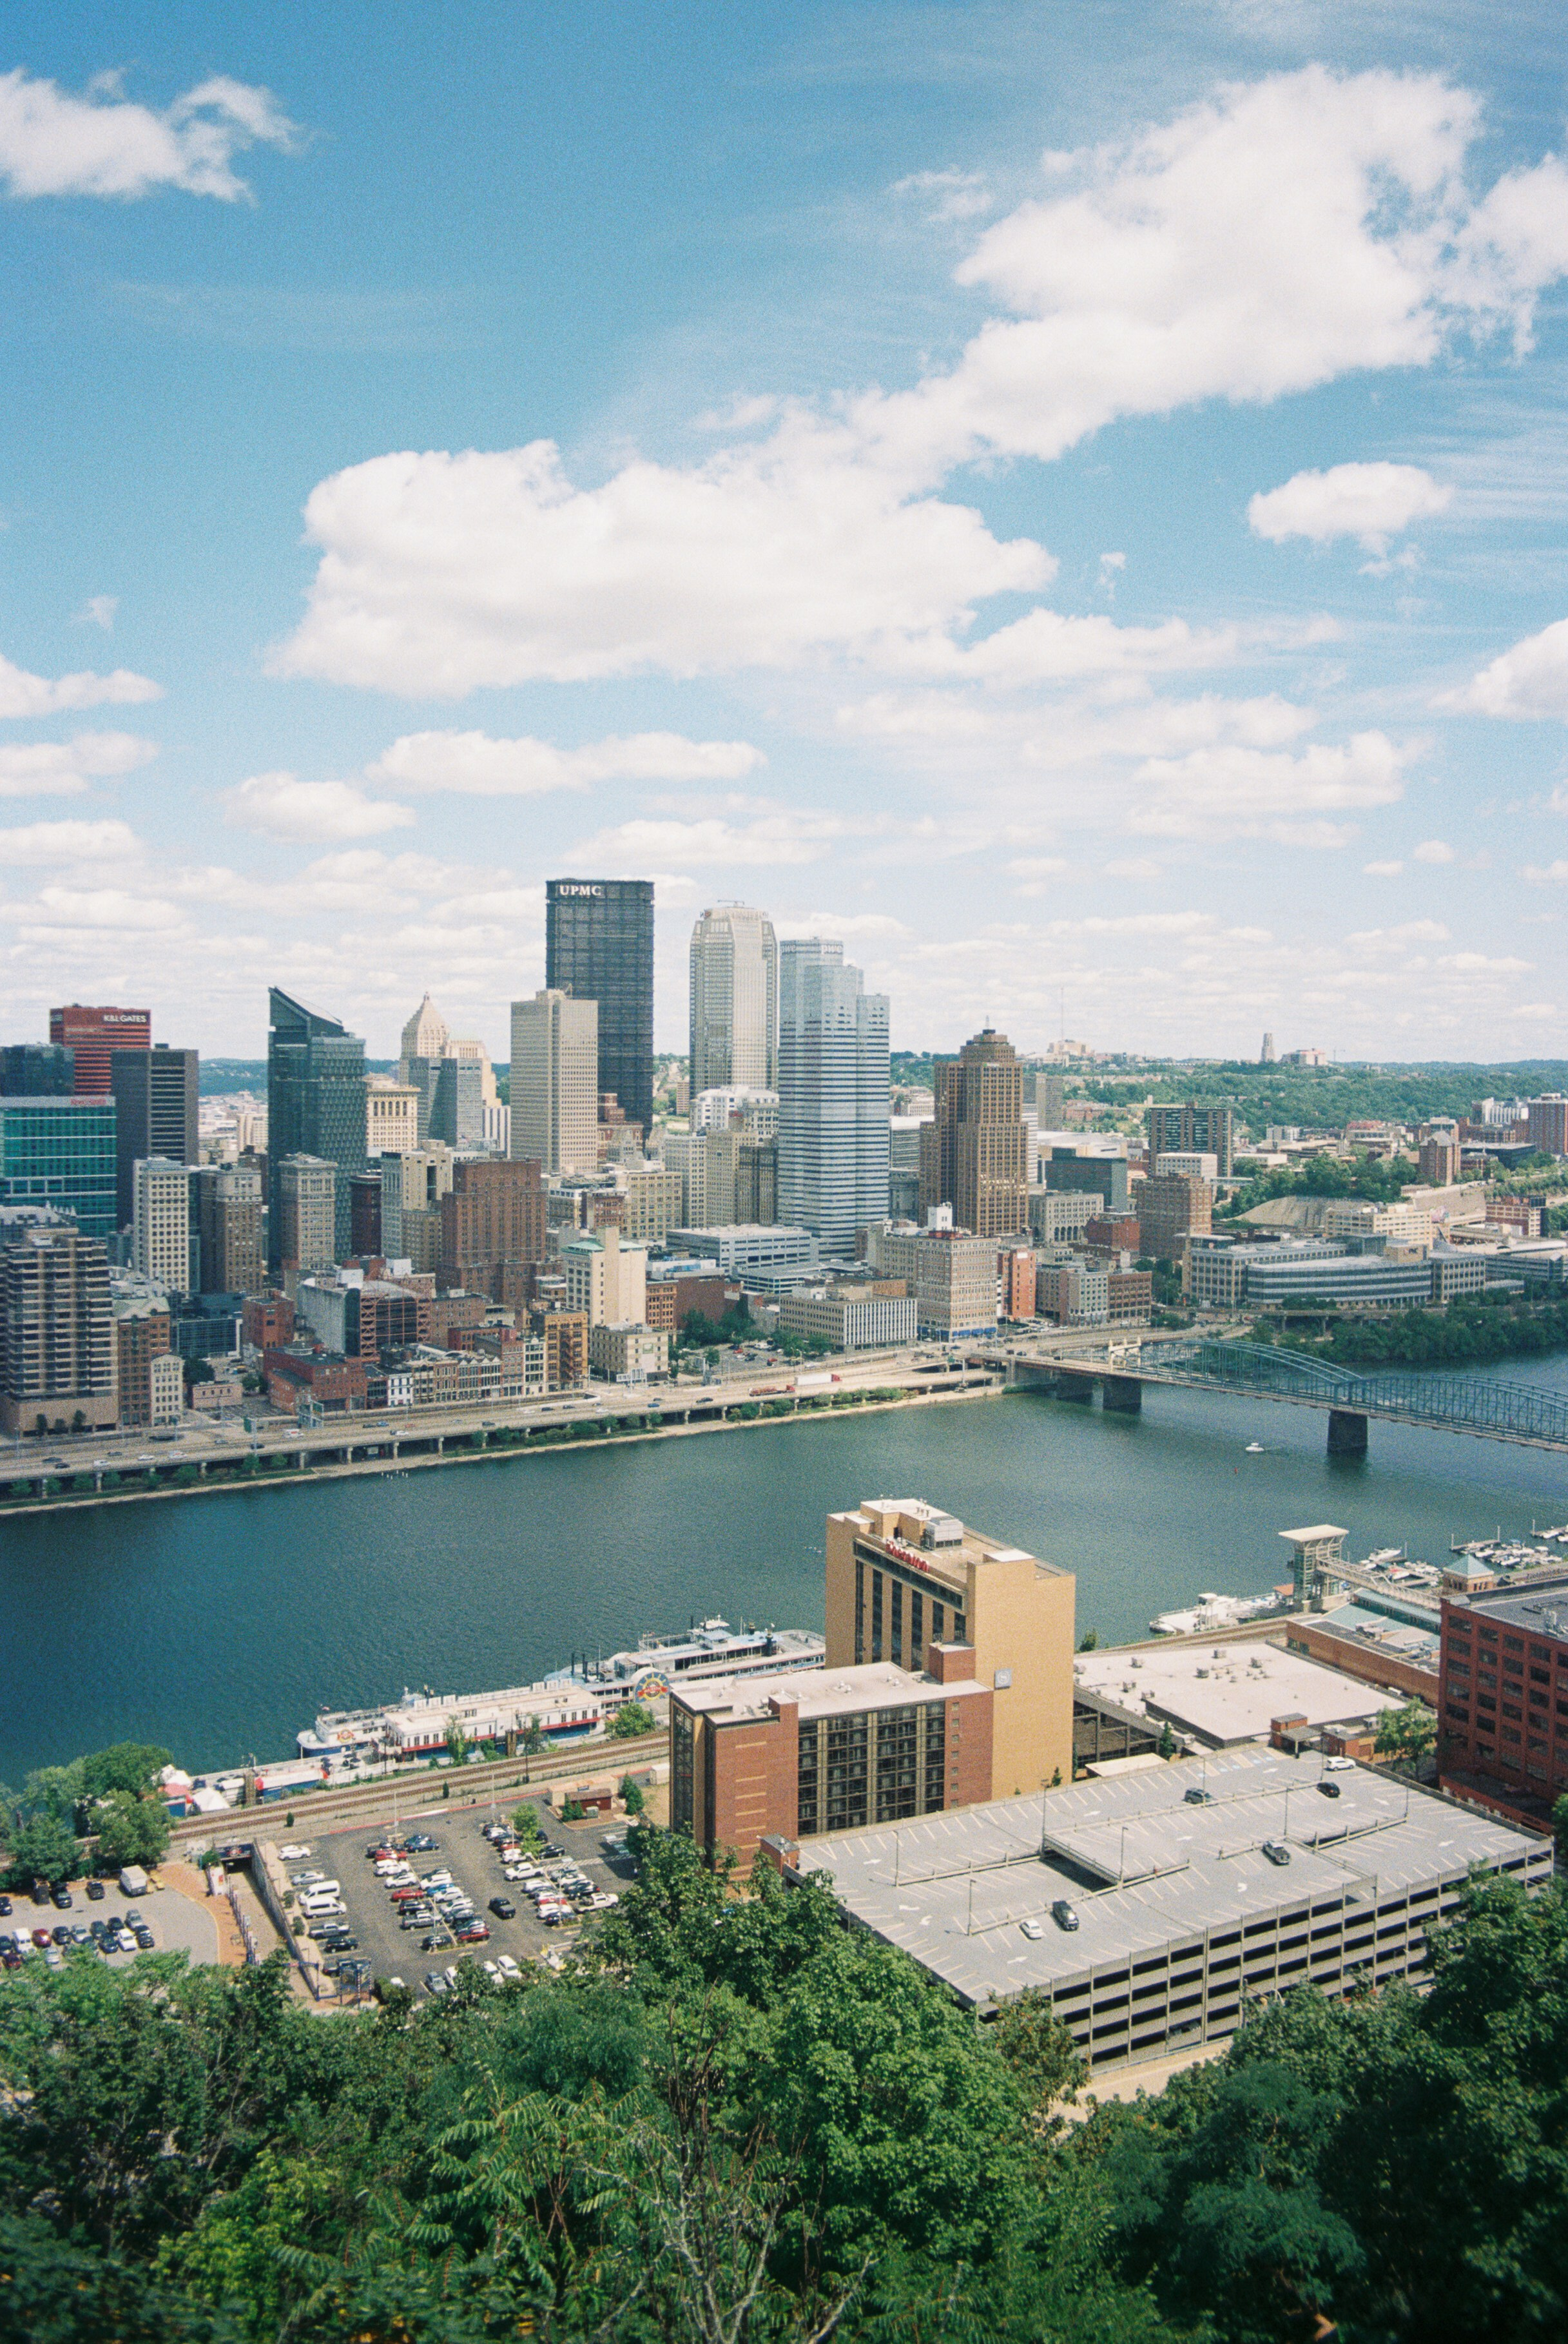
\includegraphics[scale=0.385]{./Images/banner.jpg}}} % Image background
\centering
\vspace*{5cm}
\par\normalfont\fontsize{35}{35}\sffamily\selectfont
\textbf{ECE355 Fall 2024}\\
{\LARGE Signal Analysis and Communication}\par % Book title
\vspace*{1cm}
{\Huge Nasrudeen Oladimeji}\par % Author name
\endgroup

%----------------------------------------------------------------------------------------
%	COPYRIGHT PAGE
%----------------------------------------------------------------------------------------

\newpage
~\vfill
\thispagestyle{empty}

%\noindent Copyright \copyright\ 2014 Andrea Hidalgo\\ % Copyright notice

\noindent\textsc{University of Toronto}\\

\noindent \textsc{github.com/Nasr-905}\\ % URL

\noindent Professor: Frank R. Kschischang (frank@ece.utoronto.ca)\\ % License information

\noindent \textit{First release, September 2024} % Printing/edition date

%----------------------------------------------------------------------------------------
%	TABLE OF CONTENTS
%----------------------------------------------------------------------------------------

\chapterimage{./Images/head1.jpg} % Table of contents heading image

\pagestyle{empty} % No headers

\tableofcontents % Print the table of contents itself

%\cleardoublepage % Forces the first chapter to start on an odd page so it's on the right

\pagestyle{fancy} % Print headers again

\chapterimage{./Images/head2.jpg} % Chapter heading image
\chapter{The Introduction}
\large \textbf{Administrative Information}
\begin{itemize}
    \item Quizes are weekly, except for weeks where there are midterms.
    \item 30 minutes to complete the quiz.
    \item Released on Tuesday, due on Saturday.
    \item Textbook: Alan V. Oppenheim, Alan S. Willsky with S. Hamid Nawab, Signals and Systems, Second Edition, Prentice-Hall, 1996
\end{itemize}
\begin{definition}
    [System]
    In this course, systems are devices that convert input signals to output signals.
    \[
        x(t) \to \boxed{\text{System}} \to y(t)
    \]
\end{definition}

% \chapterimage{./Images/head3.jpg} % Chapter heading image
\chapter{Signals}

\section{Introduction}

\begin{figure}[H]
    \centering
    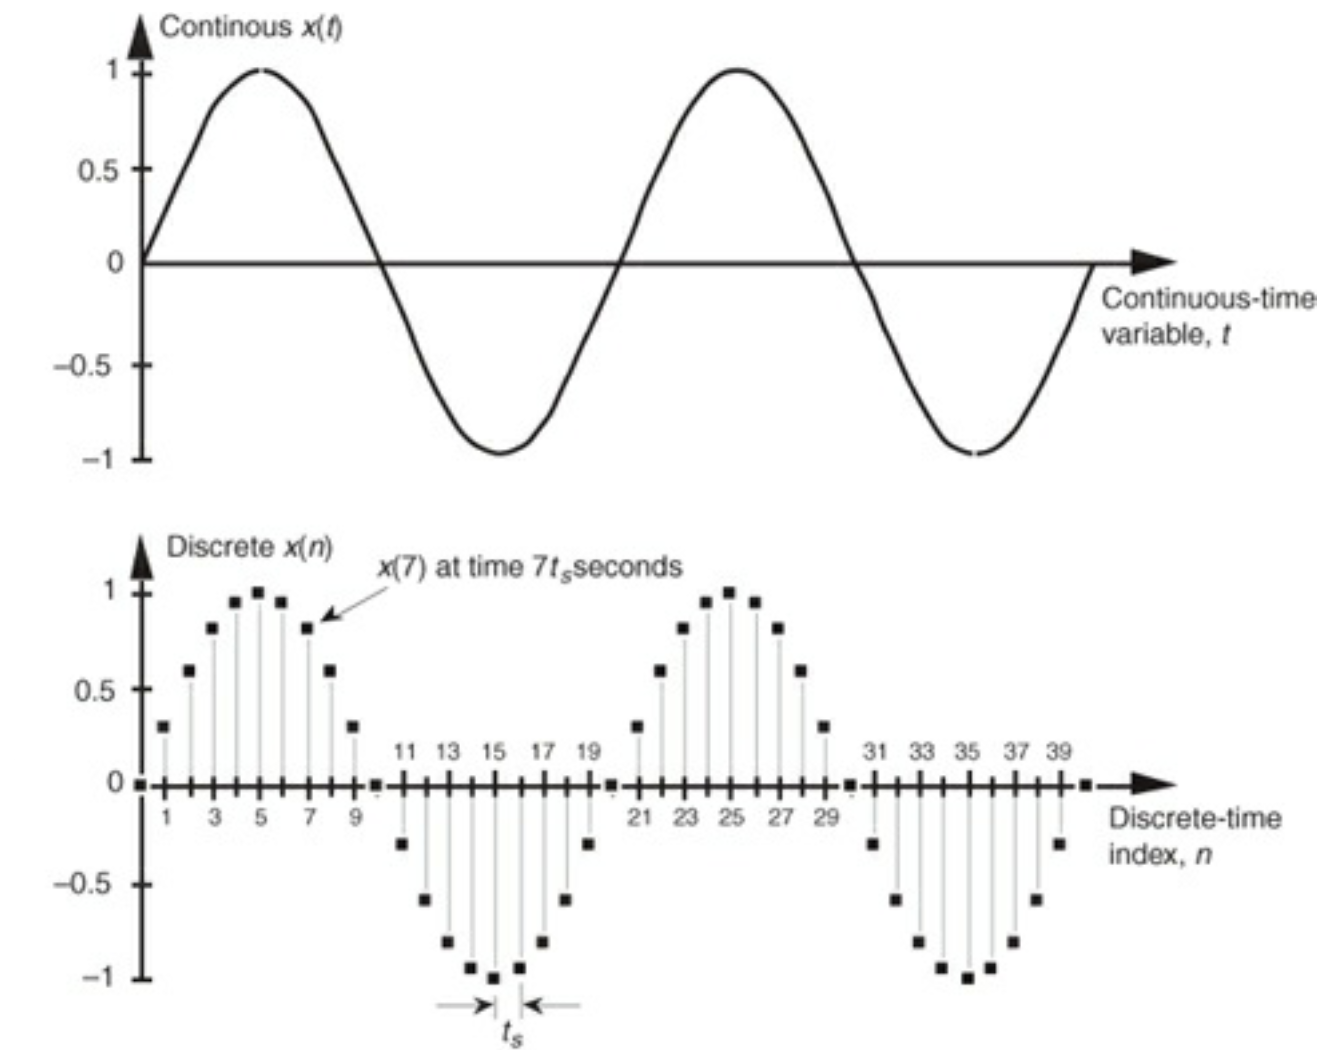
\includegraphics[width=0.5\textwidth]{./LECTURE_2/audio_5.png}
    \caption{Continuous vs. Discrete Signal}
    \label{fig:signal}
\end{figure}

\begin{definition}
    [Important Sets]
    \begin{align*}
        \mathbb{R} & = \text{Set of real numbers}     \\
        \mathbb{Z} & = \text{Set of integers}         \\
        \mathbb{N} & = \text{Set of natural numbers}  \\
        \mathbb{Q} & = \text{Set of rational numbers} \\
        \mathbb{C} & = \begin{aligned}
                           \text{Set of complex numbers} \\
                           \{a+bj : j = \sqrt{-1}\}
                       \end{aligned}
    \end{align*}
\end{definition}

\begin{definition}
    [Conjugate]
    \begin{align*}
        \text{If } z = a + bj, \text{ then } z^* = a - bj
    \end{align*}
\end{definition}

\begin{definition}
    [Magnitude]
    \begin{align*}
        \text{If } z = a + bj, \text{ then } |z| = \sqrt{a^2 + b^2} = \sqrt{z \cdot z^*}
    \end{align*}
\end{definition}

\begin{remark}
    {Containment of Sets}
    \begin{align*}
        \mathbb{N} & \subset \mathbb{Z} \subset \mathbb{Q} \subset \mathbb{R} \subset \mathbb{C}
    \end{align*}
\end{remark}

\begin{definition}
    [Signal]
    A Signal is a function of time.
    \textit{Note: This is not entirely accurate, as we'll see later in the course.}
    \begin{align*}
        x(t) & = \begin{aligned}
                     \text{Continuous signal} \\
                     \text{where } t \in \mathbb{R}
                 \end{aligned} \\
        x[n] & = \begin{aligned}
                     \text{Discrete signal} \\
                     \text{where } n \in \mathbb{Z}
                 \end{aligned}
    \end{align*}
\end{definition}

\begin{definition}
    [Function]
    A function $f:A \to B$ from a set $A$ (the domain) to a set $B$ (the co-domain) is a rule that assigns to each element $a \in A$ exactly one element $b \in B$.
\end{definition}
\begin{example}
    \begin{figure}[h]
        \centering
        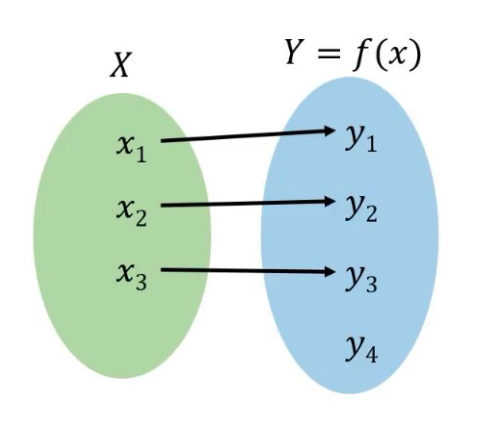
\includegraphics[width=0.5\textwidth]{./LECTURE_2/domain-range-codomain.png}
        \caption{Function}
        \label{fig:function}
    \end{figure}
    Domain of $f$, $A = \{x_1,x_2,x_3\}$, Co-domain of $f$, $B = \{y_1,y_2,y_3,y_4\}$, Range of $f$, $\{y_1,y_2,y_3\}$ (the set that contains all the images of the elements of the domain).
\end{example}

\begin{definition}
    [Range]
    The range or image of a function is the set of all possible values that the function can take. With reference to \ref{fig:function}, the range of $f$ is $\{y_1,y_2,y_3\}$.
\end{definition}

\begin{definition}
    [Inverse Image]
    The inverse image of a subset $C$ of the co-domain of a function $f$ is the set of all elements of the domain that map to the members of $C$. With reference to \ref{fig:function}, the inverse image of $\{y_1,y_2\}$ is $\{x_1,x_2\}$.
\end{definition}

\begin{definition}
    [Injective or One-to-One]
    A function $f:A \to B$ is injective if for every $b \in B$, there is at most one $a \in A$ such that $f(a) = b$. \\
    if $f(a_1) = f(a_2)$, then $a_1 = a_2$ and vice versa.
\end{definition}

\begin{figure}[h]
    \centering
    \begin{tikzpicture}
        % Define the sets
        \node (A1) at (0,3) {$A$};
        \node (A2) at (0,2) {$a_1$};
        \node (A3) at (0,1) {$a_2$};
        \node (A4) at (0,0) {$a_3$};

        \node (B1) at (4,3) {$B$};
        \node (B2) at (4,2) {$b_1$};
        \node (B3) at (4,1) {$b_2$};
        \node (B4) at (4,0) {$b_3$};
        \node (B5) at (4,-1) {$b_4$};

        % Draw arrows
        \draw[->] (A2) -- (B2);
        \draw[->] (A3) -- (B3);
        \draw[->] (A4) -- (B4);

        % Draw sets
        \draw[dashed] (-0.5,3.5) rectangle (0.5,-0.5);
        \draw[dashed] (3.5,3.5) rectangle (4.5,-1.5);
    \end{tikzpicture}
    \caption{Injective (One-to-One) Function}
    \label{fig:injective}
\end{figure}

\begin{definition}
    [Surjective or Onto]
    A function $f:A \to B$ is surjective if for every $b \in B$, there is at least one $a \in A$ such that $f(a) = b$.
    \[
        \forall b \in B, \exists a \in A \text{ such that } f(a) = b
    \]
    % figure

\end{definition}

\begin{figure}[h]
    \centering
    \begin{tikzpicture}
        % Define the sets
        \node (A1) at (0,3) {$A$};
        \node (A2) at (0,2) {$a_1$};
        \node (A3) at (0,1) {$a_2$};
        \node (A4) at (0,0) {$a_3$};
        \node (A5) at (0,-1) {$a_4$};

        \node (B1) at (4,3) {$B$};
        \node (B2) at (4,2) {$b_1$};
        \node (B3) at (4,1) {$b_2$};
        \node (B4) at (4,0) {$b_3$};

        % Draw arrows
        \draw[->] (A2) -- (B2);
        \draw[->] (A3) -- (B3);
        \draw[->] (A4) -- (B4);
        \draw[->] (A5) -- (B2);

        % Draw sets
        \draw[dashed] (-0.5,3.5) rectangle (0.5,-1.5);
        \draw[dashed] (3.5,3.5) rectangle (4.5,-0.5);
    \end{tikzpicture}
    \caption{Surjective (Onto) Function}
    \label{fig:surjective}
\end{figure}

\begin{definition}
    [Bijective]
    A function $f:A \to B$ is bijective if it is both injective and surjective.

\end{definition}
\begin{figure}[h]
    \centering
    \begin{tikzpicture}
        % Define the sets
        \node (A1) at (0,3) {$A$};
        \node (A2) at (0,2) {$a_1$};
        \node (A3) at (0,1) {$a_2$};
        \node (A4) at (0,0) {$a_3$};

        \node (B1) at (4,3) {$B$};
        \node (B2) at (4,2) {$b_1$};
        \node (B3) at (4,1) {$b_2$};
        \node (B4) at (4,0) {$b_3$};

        % Draw arrows
        \draw[->] (A2) -- (B2);
        \draw[->] (A3) -- (B3);
        \draw[->] (A4) -- (B4);

        % Draw sets
        \draw[dashed] (-0.5,3.5) rectangle (0.5,-0.5);
        \draw[dashed] (3.5,3.5) rectangle (4.5,-0.5);
    \end{tikzpicture}
    \caption{Bijective (One-to-One and Onto) Function}
    \label{fig:bijective}
\end{figure}
\end{document}

% \chapter{More Functions}

\begin{corollary}
    [Functions of the Co-domain]
    \[
        f:A \to B \qquad g: B \to C
    \]
    % draw the set diagrams
    \begin{figure}
        \centering
        \begin{tikzpicture}
            % Define the sets
            \node (A1) at (0,3) {$A$};
            \node (A2) at (0,2) {$a_1$};
            \node (A3) at (0,1) {$a_2$};
            \node (A4) at (0,0) {$a_3$};
            \node (A5) at (0,-1) {$a_4$};

            \node (B1) at (4,3) {$B$};
            \node (B2) at (4,2) {$b_1$};
            \node (B3) at (4,1) {$b_2$};
            \node (B4) at (4,0) {$b_3$};
            \node (B5) at (4,-1) {$b_4$};

            \node (C1) at (8,3) {$C$};
            \node (C2) at (8,2) {$c_1$};
            \node (C3) at (8,1) {$c_2$};
            \node (C4) at (8,0) {$c_3$};
            \node (C5) at (8,-1) {$c_4$};

            % Draw arrows
            \draw[->] (A2) -- (B2);
            \draw[->] (A3) -- (B3);
            \draw[->] (A4) -- (B4);
            \draw[->] (A5) -- (B5);

            \draw[->] (B2) -- (C2);
            \draw[->] (B3) -- (C3);
            \draw[->] (B4) -- (C4);
            \draw[->] (B5) -- (C5);

            % Draw sets
            \draw[dashed] (-0.5,3.5) rectangle (0.5,-1.5);
            \draw[dashed] (3.5,3.5) rectangle (4.5,-1.5);
            \draw[dashed] (7.5,3.5) rectangle (8.5,-1.5);
        \end{tikzpicture}
        \caption{Functions of the Co-domain}
        \label{fig:co-domain}

    \end{figure}
\end{corollary}

\begin{definition}
    [Powers of Sets]
    The set of all functions from $A$ to $B$ is denoted by $B^A$.
\end{definition}

\begin{example}
    [Powers of Sets]
    if $A = \{1, 2\}$ and $B = \{x,y,z\}$, then $B^A$ has $3^2 = 9$ elements.
\end{example}

\begin{example}
    [Powers of Sets 2]
    \begin{align*}
        f & = \begin{matrix}
                  1    & 2    \\
                  f(1) & f(2)
              \end{matrix} \\ B^A &= \{ \begin{matrix}
            1 & 2 \\
            x & x
        \end{matrix}, & \begin{matrix}
            1 & 2 \\
            x & y
        \end{matrix}, & \begin{matrix}
            1 & 2 \\
            x & z
        \end{matrix} \\ \begin{matrix}
            1 & 2 \\
            y & x
        \end{matrix} & \begin{matrix}
            1 & 2 \\
            y & y
        \end{matrix} & \begin{matrix}
            1 & 2 \\
            y & z
        \end{matrix} \\ \begin{matrix}
            1 & 2 \\
            z & x
        \end{matrix} & \begin{matrix}
            1 & 2 \\
            z & y
        \end{matrix} & \begin{matrix}
            1 & 2 \\
            z & z
        \end{matrix}\}
    \end{align*}
\end{example}

\section{The Complex Exponential Function}

\begin{definition}
    [The Complex Exponential Function]
    \begin{align*}
        \exp : \mathbb{C} & \to \mathbb{C} \quad \text{via}                                                                         \\
        z                 & \mapsto \exp(z) = 1 + z + \frac{z^2}{2!} + \frac{z^3}{3!} + \cdots = \sum_{n=0}^{\infty} \frac{z^n}{n!}
    \end{align*}
    $exp$ is an entire function, so the taylor series converges for all $z \in \mathbb{C}$.
\end{definition}
\begin{proof}
    Apply the ratio test to prove that the series converges at all $z \in \mathbb{C}$.
\end{proof}

\begin{example}
    [Euler's Relation]
    Say $z = j\theta | \theta \in \mathbb{R}$
    \begin{align*}
        \exp(j\theta) & = 1 + j\theta - \frac{\theta^2}{2!} - j\frac{\theta^3}{3!} + \frac{\theta^4}{4!} + j\frac{\theta^5}{5!} + \cdots            \\
                      & = (1 - \frac{\theta^2}{2!} + \frac{\theta^4}{4!} - \cdots) + j(\theta - \frac{\theta^3}{3!} + \frac{\theta^5}{5!} - \cdots) \\
                      & = \cos(\theta) + j\sin(\theta)
    \end{align*}

\end{example}

\begin{definition}
    [Principle Argument]
    The principle argument of $z \in \mathbb{C}$ is denoted by $\arg(z)$ and is defined as the angle between the positive real axis and the line segment from the origin to $z$.
    \[
        -\pi < \arg(z) = \theta \leq \pi \quad \text{where} \quad \theta = |z| \exp(j\theta)
    \]
\end{definition}

\begin{definition}
    [Polar form Conjugation]
    \[
        \overline{z} = |z| \exp(-j\theta) = x - jy \quad \text{where} \quad z = x + jy
    \]
\end{definition}

\section{Signals}
\subsection*{Four Types of Signals}
\begin{enumerate}
    \item Discrete-Time Signals
    \item \begin{enumerate}
              \item $\mathbb{R}^{\mathbb{Z}}$ Real-valued signals
              \item $\mathbb{C}^{\mathbb{Z}}$ Complex-valued signals
          \end{enumerate}
    \item Continuous-Time Signals
    \item \begin{enumerate}
              \item $\mathbb{R}^{\mathbb{R}}$ Real-valued signals
              \item $\mathbb{C}^{\mathbb{R}}$ Complex-valued signals
          \end{enumerate}
\end{enumerate}

\begin{example}
    [Real-Valued Signals]
    \[x : \mathbb{R} \to \mathbb{R} \qquad\qquad y : \mathbb{Z} \to \mathbb{R}\]
    \begin{figure}
        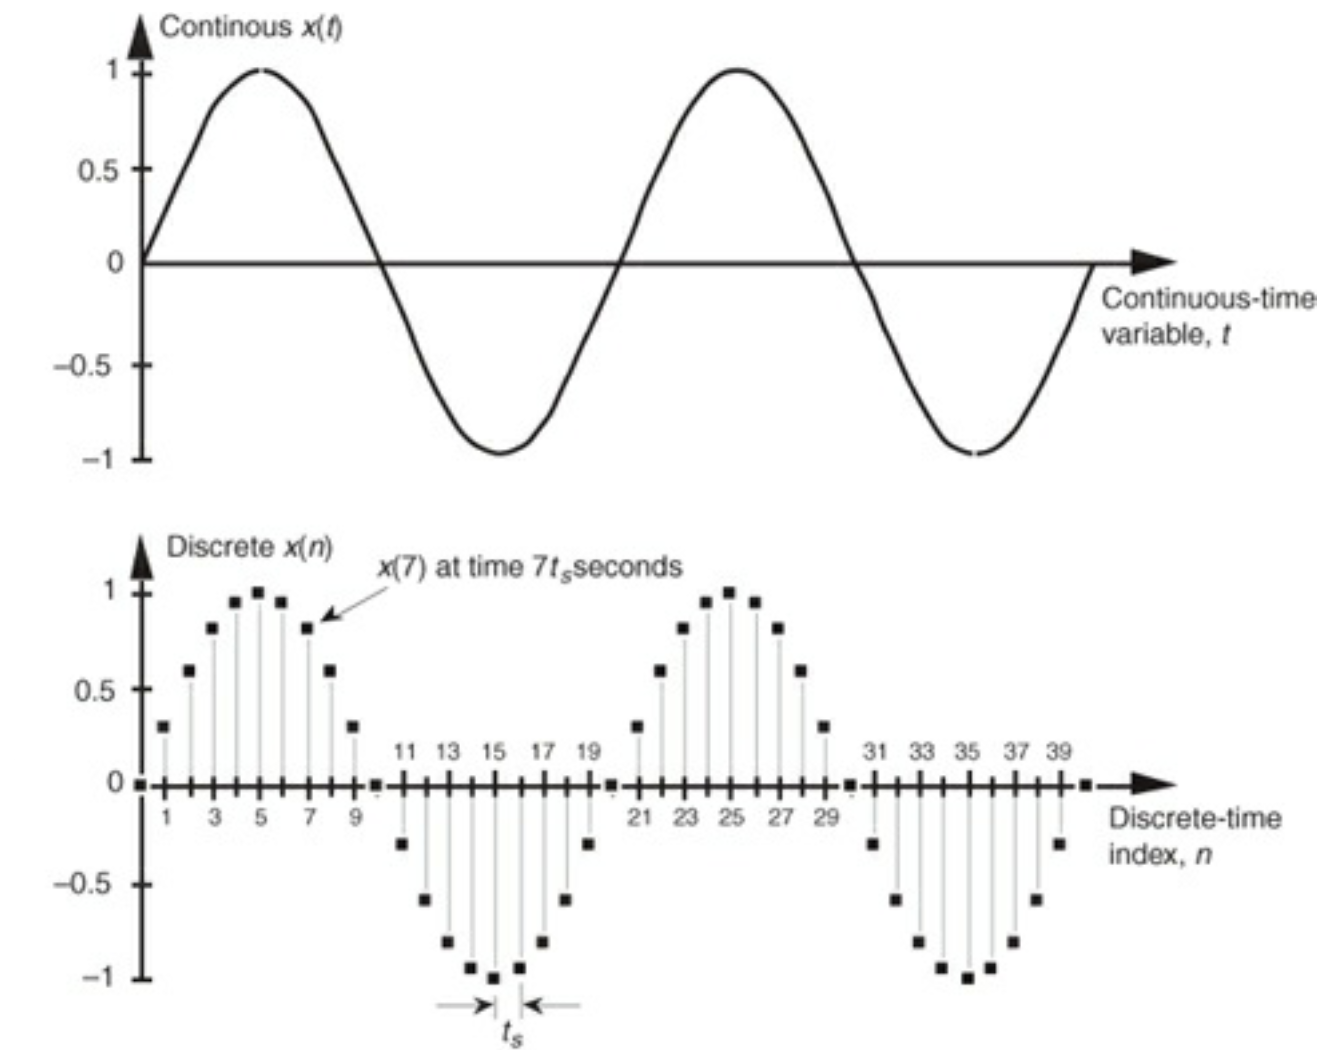
\includegraphics[scale=1]{./LECTURE_2/audio_5.png}
        \caption{Real-Valued Signals}
    \end{figure}
    \[x(t) \qquad \qquad x[t]\]
\end{example}
\begin{definition}
    [Support]
    The \textit{support} of a nonzero signl $x \in \mathbb{C}^\mathbb{R}$ is the smallest interval $[a,b]$ such that $x(t) = 0$ for all $t \notin [a,b]$. \\
    Essentially, the support is the set of all $t$ such that $x(t) \neq 0$.
    IMAGE
\end{definition}

\begin{definition}
    [Energy]
    The \textit{energy} of a signal $x \in \mathbb{C}^\mathbb{R}$ is defined as
    \[
        E_x = \int_{-\infty}^{\infty} |x(t)|^2 dt
    \]
    If $x \in \mathbb{C}^\mathbb{R}$
    \[
        E_x = \int_{t=-\infty}^{\infty} |x(t)|^2
    \]
\end{definition}

\begin{definition}
    [Average Power]
    The \textit{average power} of a signal $x \in \mathbb{C}^\mathbb{R}$ is defined as
    \[
        P_x = \lim_{T \to \infty} \frac{1}{2T} \int_{-T}^{T} |x(t)|^2 dt
    \]
\end{definition}


% simple circuit with voltage source and resistor
% \begin{figure}
%     \centering
%     \begin{circuitikz}
%         \draw (0,0) to[V, v=$V_s$] (0,2) to[R, l=$R$] (2,2) to[short] (2,0) to[short] (0,0);
%     \end{circuitikz}
%     \caption{Simple Circuit}
%     \label{fig:simple-circuit}
% \end{figure}

\begin{remark}
    Homework is assigned!
\end{remark}

% \chapter{Supports}

\begin{definition}
    [Support of a Function of a continuous variable]
    The support of a function $f(t)$ of a continuous variable $t$ is the smallest time interval $[a,b]$ for which $f(t) \neq 0$.
\end{definition}

\begin{definition}
    [Support of  a function of a discrete variable]
    The support of a function $f[n]$ of a discrete variable $n$ is the smallest set of integers $n$ for which $f[n] \neq 0$.
\end{definition}

\begin{definition}
    [Energy of a Continuous-time Signal]
    The energy of a continuous-time signal $x(t)$ is defined as
    \[
        E_x = \int_{-\infty}^{\infty} |x(t)|^2 dt
    \]

\end{definition}

\begin{definition}
    [Energy of a Discrete-time Signal]
    The energy of a discrete-time signal $x[n]$ is defined as
    \[
        E_x = \sum_{n=-\infty}^{\infty} |x[n]|^2
    \]
\end{definition}
\begin{remark}
    Energies of a signal are \textbf{always positive}, but may not exist (i.e. be infinite)
\end{remark}

\begin{figure}[H]
    \centering
    \begin{circuitikz}
        \draw (0,0) to[V, v=$V_s$] (0,2) to[R, l=$1 \Omega$] (2,2) to[short] (2,0) to[short] (0,0);
    \end{circuitikz}
\end{figure}
\begin{observation}
    A signal of finite energy is called an energy signal.
\end{observation}
\section{Power}
\begin{definition}
    [Average Power of a Continuous-time Signal]
    The average power of a continuous-time signal $x(t) \in \mathbb{C}^\mathbb{R}$ is defined as (if it exists):
    \[
        P_x = \lim_{T \to \infty} \frac{1}{2T} \int_{-T}^{T} |x(t)|^2 dt
    \]
\end{definition}

\begin{definition}
    [Average Power of a Discrete-time Signal]
    The average power of a discrete-time signal $x[n] \in \mathbb{C}^\mathbb{Z}$ is defined as (if it exists):
    \[
        P_x = \lim_{N \to \infty} \frac{1}{2N+1} \sum_{n=-N}^{N} |x[n]|^2
    \]
\end{definition}


\begin{definition}
    [Power Signal]
    A signal $x(t)$ is a power signal if $0 < P_x < \infty$. In other words, the average power of the signal is finite.
\end{definition}
\begin{corollary}
    Every energy signal has zero average power.
\end{corollary}

\begin{example}
    [Energy of the Zero Signal]
    \begin{align}
        \text{zero}(t) & = 0 \quad \forall t \in \mathbb{R} \\
        \text{zero}[n] & = 0 \quad \forall n \in \mathbb{Z}
    \end{align}
    \begin{align}
        USE THE EQUATIONS
    \end{align}
\end{example}

\begin{example}
    [Energy of the Rectangular Pulse]
    \begin{align}
        \text{rect}(t) & = \begin{cases}
                               1 & |t| < \frac{1}{2} \\
                               0 & \text{otherwise}
                           \end{cases} \\
        \text{rect}[n] & = \begin{cases}
                               1 & |n| < \frac{1}{2} \\
                               0 & \text{otherwise}
                           \end{cases}
    \end{align}
    % figure of the rectangular pulse
    \begin{figure}[H]
        \centering
        % tikz figure
        \begin{tikzpicture}
            \draw[->] (-2,0) -- (2,0) node[right] {$t$};
            \draw[->] (0,0) -- (0,1.5) node[above] {$\text{rect}(t)$};
            \draw (-1,0) -- (-1,1) -- (1,1) -- (1,0);
        \end{tikzpicture}
        \caption{Rectangular Pulse}
    \end{figure}
    \begin{align}
        \int_{-\infty}^{\infty} |\text{rect}(t)|^2 dt & = \int_{-\frac{1}{2}}^{\frac{1}{2}} 1^2 dt = 1 \\
        \sum_{n=-\infty}^{\infty} |\text{rect}[n]|^2  & = \sum_{n=-\frac{1}{2}}^{\frac{1}{2}} 1^2 = 1
    \end{align}
\end{example}

\begin{example}
    Find the power of $s (t) = \cos(\frac{2\pi t}{T}) : T > 0, A > 0$ \\
    \begin{align}
        P_s & = \lim_{T \to \infty} \frac{1}{2T} \int_{-T}^{T} |\cos(\frac{2\pi t}{T})|^2 dt                                                                                              \\
            & = \lim_{T \to \infty} \frac{1}{2T} \int_{-T}^{T} \cos^2(\frac{2\pi t}{T}) dt                                                                                                \\
            & = \lim_{T \to \infty} \frac{1}{2T} \int_{-T}^{T} \frac{1 + \cos(\frac{4\pi t}{T})}{2} dt                                                                                    \\
            & = \lim_{T \to \infty} \frac{1}{2T} \left[ \frac{t}{2} + \frac{T}{4\pi} \sin(\frac{4\pi t}{T}) \right]_{-T}^{T}                                                              \\
            & = \lim_{T \to \infty} \frac{1}{2T} \left[ \frac{T}{2} + \frac{T}{4\pi} \sin(\frac{4\pi T}{T}) - \left( -\frac{T}{2} - \frac{T}{4\pi} \sin(\frac{4\pi T}{T}) \right) \right] \\
            & = \lim_{T \to \infty} \frac{1}{2T} \left[ T + \frac{T}{2\pi} \sin(4\pi) + T + \frac{T}{2\pi} \sin(-4\pi) \right]                                                            \\
            & = \lim_{T \to \infty} \frac{1}{2T} \left[ 2T \right] = 1
    \end{align}
\end{example}

% \chapter{}

\section{Zero-energy Signals}

\begin{claim}
    Discrete-time $\text{zero}[n]$ is a zero-energy signal. There are no other zero-energy signals.
\end{claim}

\begin{proof}
    If $x[n] \neq 0$, then $x^2[n] > 0$ for at least one $n$. Thus, $\sum_{n=-\infty}^{\infty} x^2[n] > 0$. Because there's no negative energy, you can't cancel positive energy.
\end{proof}

\section{Energy in Continuous-time}

\begin{claim}
    $\text{zero}(t)$ has zero energy, but there exists other zero-energy signals.
    \[
        x(t) = \begin{cases}
            1 & \text{if } t = 0 \\
            0 & \text{otherwise}
        \end{cases}
    \]
\end{claim}


\begin{tikzpicture}
    \begin{axis}[
            xlabel=$t$,
            ylabel=$x(t)$,
            axis lines=middle,
            xmin=-2, xmax=2,
            ymin=-0.5, ymax=1.5,
            xtick={-1,0,1},
            ytick={0,1},
            yticklabels={0,1},
            xticklabels={$-1$,0,$1$},
            samples=100,
            smooth,
            thick
        ]
        \addplot+[domain=-2:2] {ifthenelse(abs(x-0)<0.01, 1, 0)};
        % point at (0,1)
        \addplot+[mark=*,mark options={fill=white}] coordinates {(0,1)};
        % hole at (0,0)
        \addplot+[mark=*,mark options={fill=white}] coordinates {(0,0)};
    \end{axis}
\end{tikzpicture}
\begin{definition}
    [Zero Energy Function]
    We define the \textbf{zero energy function} as
    \begin{align*}
        x_\delta(t) = \begin{cases}
                          1 & \text{if } |t| \leq \Delta \\
                          0 & \text{otherwise}
                      \end{cases}
    \end{align*}
    Then the energy of $x_\delta(t)$ is given by $E_\Delta = 2\Delta$. \\
    So as $\Delta \to 0$, $E_\Delta \to 0$ and $x_\Delta \to 0$.
\end{definition}

\begin{remark}
    \begin{itemize}
        \item A signal of a finite number of impulses will have zero energy.
        \item A signal with a countable infinite number of impulses will have zero energy.
        \item A signal with an uncountable infinite number of impulses will have non-zero energy.
              \begin{itemize}
                  \item Example: $x(t) = \begin{cases}
                                1 & \text{if } t \in \mathbb{Q} \\
                                0 & \text{otherwise}
                            \end{cases}$.
                  \item this may be in the wrong place...
              \end{itemize}
    \end{itemize}
\end{remark}

\begin{vocabulary}
    [Zero Energy Functions]
    If $x(t)$ is a zero-energy function, then we say that $x(t) = \text{zero}(t)$ almost everywhere.
\end{vocabulary}

\begin{vocabulary}
    [Signal Equivalence]
    Say $x(t) = y(t)$ almost everywhere if $x(t) - y(t) = \text{zero}(t)$ almost everywhere.
\end{vocabulary}

\section{Signal Spaces}
\begin{remark}
    \underline{Signal spaces are vector spaces! And signals are vectors!}
\end{remark}

\begin{definition}
    [Signal Addition]
    Given two signals $x, y \in \mathbb+
    {D}$ we can define a new signal $(x+y)$\end{definition}

\begin{remark}
    The addition o two signal sis always a signal
\end{remark}

\section{}

% \chapter{Affine Transformations of the Independent Variable (Oppenheim 1.2-1.3)}

\begin{definition}
    [Affine Transformation]
    An \textbf{affine transformation} of the independent variable is a transformation of the form
    \[
        y(t) = x(at + b)
    \]
    where $a$ and $b$ are constants.
\end{definition}

\begin{definition}
    [Time Reversal]
    The \textbf{time reversal} of a signal $x(t)$ is defined as
    \[
        x(t) \to x(-t) = \tilde{x}(t)
    \]
\end{definition}
\begin{figure}[h]
    \centering
    \begin{minipage}{0.45\textwidth}
        \centering
        \begin{tikzpicture}[scale=0.8]
            % Original signal x(t)
            \begin{axis}[
                    title={Original Signal $x(t)$},
                    xlabel={$t$},
                    ylabel={$x(t)$},
                    axis lines=middle,
                    grid=both,
                    width=10cm,
                    height=6cm,
                    domain=-5:5,
                    samples=100
                ]
                \addplot[blue, thick] {sin(deg(x))};
            \end{axis}
        \end{tikzpicture}
    \end{minipage}
    \hfill
    \begin{minipage}{0.45\textwidth}
        \centering
        \begin{tikzpicture}[scale=0.8]
            % Time-reversed signal x(-t)
            \begin{axis}[
                    title={Time-Reversed Signal $x(-t)$},
                    xlabel={$t$},
                    ylabel={$x(-t)$},
                    axis lines=middle,
                    grid=both,
                    width=10cm,
                    height=6cm,
                    domain=-5:5,
                    samples=100
                ]
                \addplot[red, thick] {sin(deg(-x))};
            \end{axis}
        \end{tikzpicture}
    \end{minipage}
    \caption{Time Reversal of a Signal}
    \label{fig:time-reversal}
\end{figure}

\begin{definition}
    [Time Dilations]
    The \textbf{time dilation} of a signal $x(t)$ is defined as
    \[
        x(t) \to x(at)
    \]
\end{definition}

\begin{definition}
    [Time Advancement]
    The \textbf{time advancement} of a signal $x(t)$ is defined as
    \[
        x(t) \to x(t - b)
    \]
\end{definition}

\begin{definition}
    [Time Delay]
    The \textbf{time delay} of a signal $x(t)$ is defined as
    \[
        x(t) \to x(t + b)
    \]
\end{definition}

\begin{corollary}
    [Time Dilation in Discrete-time]
    The time dilation of a discrete-time signal $x[n]$ is defined as
    \[
        x[n] \to x[an]
    \]
    Where $1< |a| \in \mathbb{Z}$ \\
    $x[n/2]$ Doesn't make sense because $x[1/2], x[3/2], \ldots$ are not defined.
\end{corollary}

\begin{definition}
    [periodic in Continuos-time]
    A signal $x(t)$ is \textbf{T-periodic} with period $T$ if:
    \[
        x(t) = x(t + T) \quad \forall t \in \mathbb{R}
    \]
\end{definition}

\begin{definition}
    [the fundemental period]
    The \textbf{fundamental period} of a signal $x(t)$ is the smallest $T$ such that $x(t)$ is $T$-periodic.
\end{definition}

\begin{definition}
    [periodic in Discrete-time]
    A signal $x[n]$ is \textbf{N-periodic} with period $N$ if:
    \[
        x[n] = x[n + N] \quad \forall n \in \mathbb{Z}
    \]
\end{definition}

\begin{definition}
    [Even Signal]
    A signal $x(t)$ is \textbf{even} if
    \[
        x(t) = \tilde{x}(t) = x(-t) \quad \forall t \in \mathbb{R}
    \]
\end{definition}

\begin{definition}
    [Odd Signal]
    A signal $x(t)$ is \textbf{odd} if
    \[
        x(t) = -\tilde{x}(t) = -x(-t) \quad \forall t \in \mathbb{R}
    \]
\end{definition}

\begin{theorem}
    [Even and Odd Decomposition]
    Any signal $x(t)$ can be decomposed into an even part $x_e(t)$ and an odd part $x_o(t)$ as follows:
    \[
        x(t) = x_{even}(t) + x_{odd}(t)
    \]
    where
    \begin{align*}
        x_{even}(t) & = \frac{1}{2} \left[ x(t) + x(-t) \right] \\
        x_{odd}(t)  & = \frac{1}{2} \left[ x(t) - x(-t) \right]
    \end{align*}
\end{theorem}
% tikz square wave example
\begin{figure}
    \centering
    \begin{tikzpicture}
        % square wave

        \draw[thick] (0, 1) -- (1, 1) -- (1, 0);
        % axis
        \draw[->] (-0.5,0) -- (1.5,0) node[right] {$t$};
        \draw[->] (0,-0.5) -- (0,1.5) node[above] {$x(t)$};

        % even part

        \draw[thick] (4, 0) -- (4, 0.5) -- (6, 0.5) -- (6, 0);

        \draw[->] (3.5,0) -- (6.5,0) node[right] {$t$};
        \draw[->] (3.5,0) -- (6.5,0) node[below] {Even};
        \draw[->] (5,-0.5) -- (5,1.5) node[above] {$x(t)$};

        % odd part

        \draw[thick] (8, 0) -- (8, -0.5) -- (9, -0.5) -- (9, 0.5) -- (10, 0.5) -- (10, 0);

        \draw[->] (7.5,0) -- (10.5,0) node[right] {$t$};
        \draw[->] (7.5,0) -- (10.5,0) node[below] {Odd};
        \draw[->] (9,-0.5) -- (9,1.5) node[above] {$x(t)$};


    \end{tikzpicture}
\end{figure}


\section{Complex Exponential Signals}

\begin{definition}
    [Complex Exponential Signal]
    A \textbf{complex exponential signal} is defined as
    \[
        x(t) = e^{st} \in \mathbb{C}^{\mathbb{R}}
    \]
    where $A, s \in \mathbb{C}$ and $t \in \mathbb{R}$. \\

\end{definition}

\end{document}